% /*\part{Introduction to Operating System}
% \newpage*/
\chapter{What is Operating System?}

Operating System is a combination of two parts:

\begin{itemize}
    \item Hardware;
    \item Software;
\end{itemize}

Operating System is a program that acts as intermediary between a user of a computer and the computer hardware.

The main goal of OS are:

\begin{itemize}
    \item Execute user program and make solving user problems easier;
    \item Use the computer hardware in an efficient manner;
    \item Make the computer system easier to use;
\end{itemize}

To sum up, an OS provides an environment in which other software can do
useful work.
A computer System consists on 4 components: HW, SO, Applications and
Users.
The Operating System coordinates Hardware and Applications.
An OS is also a resource allocator (it manages all resources), and a control program (it controls
the execution of programs to prevent errors and improper use of the computer).

\begin{figure}[htbp]
    \centering
    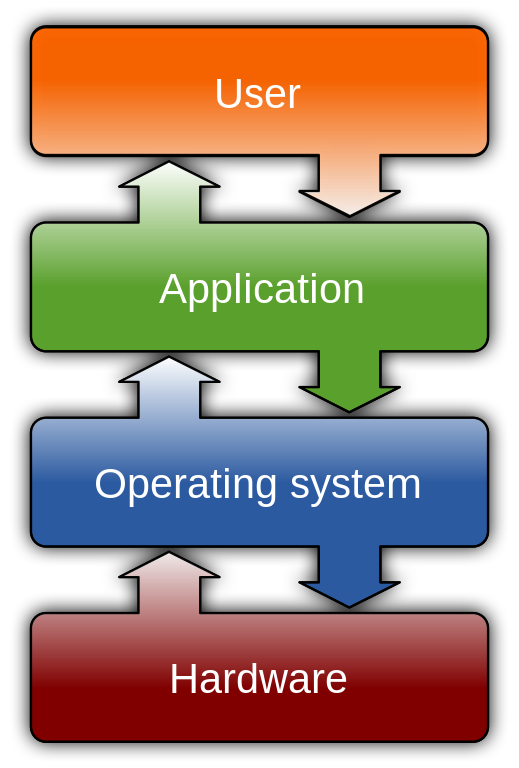
\includegraphics[scale=0.2]{img/Operating_system.png}
    % \caption{Propagazione onde elettromagnetiche}
    % \label{OndeElettromagentiche}
\end{figure}

\newpage
\section{Computer System}
A Computer system when booted up launches a procedure called bootstrap which launches the
OS kernel and starts execution.

\begin{figure}[htbp]
    \centering
    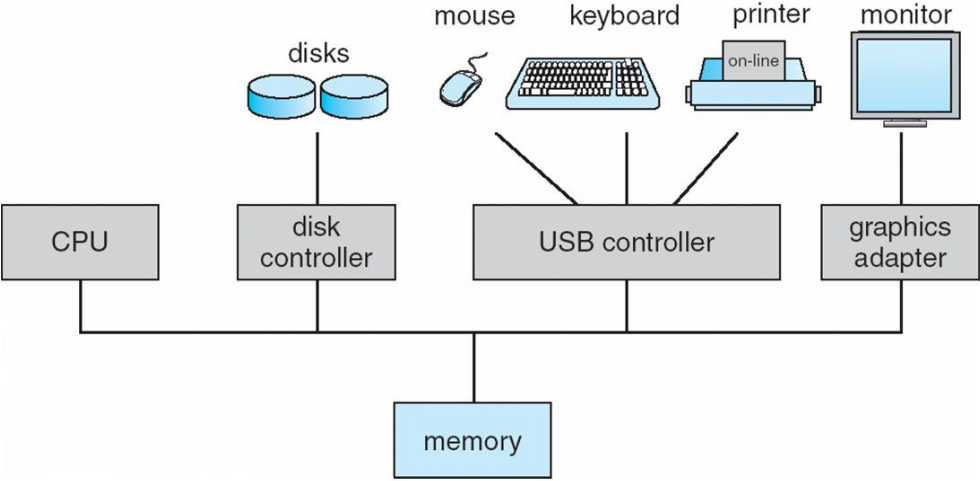
\includegraphics[scale=0.30]{img/cs.png}
\end{figure}

\subsection{How do all these things work together?}
Device controller informs the
CPU that it has finished its
operation by causing an
interrupt, an event in the OS.

\begin{figure}[htbp]
    \centering
    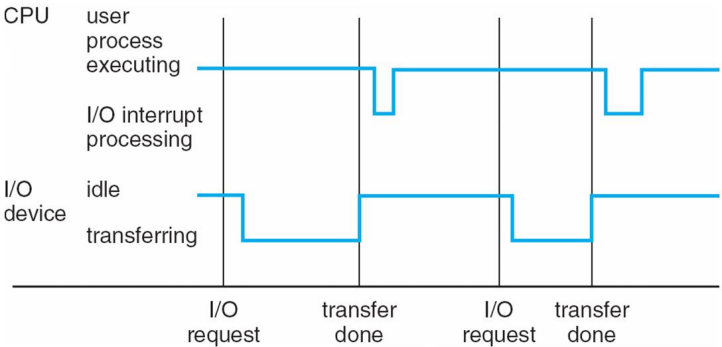
\includegraphics[scale=0.45]{img/inter.png}
\end{figure}

Example: when you try to
transfer data, the CPU is
notified when the device (may
be a pen drive) has finished to
transfer all the data through a
message of interrupt.

Every interrupt message has a memory address associated. The table that determines all of these
addresses is generated at startup.
When an interrupt occurs, the CPU saves the current Program Counter (PC) value and jumps to
the first instruction of the routine to handle the interrupt, executes the routine and then jumps
back to where the PC was. We can say that an OS is interrupt driven.

What if the CPU is doing something very important when an interrupt message arrives?
There are two types of interrupt:

\begin{itemize}
    \item Maskable interrupts: can be handled whenever critical instructions are being executed;
    \item Non-maskable interrupts: have high priority and have to be handled right as they arrive;
\end{itemize}

The structure of interrupt implies that CPU has to manage I/O processes after the transfer of each
portion of data has been executed, we don’t want that.
The DMA (Direct Memory Access) manages the data transfer and notifies the CPU only after
everything is finished

\newpage
\section{Memory}

\begin{itemize}
    \item \textbf{Cache - SRAM}: it is really fast but expensive (1 ns latency). It’s the first memory che CPU checks when
searching for a piece of information. It is \textit{volatile};
    \item \textbf{Main memory - DRAM}: large storage media that the CPU can access directly (DRAM), typically volatile
(20 ns latency). It is \textit{volatile};
    \item \textbf{Secondary storage - HDD/Flash NAND}: extensions of the main memory (non volatile) such as HDD and SSD
($250\,000$ ns latency). It is  \textit{not volatile};
\end{itemize}

\textbf{Caching}: copying information into faster storage system. Main memory can be viewed as a cache
for secondary storage.
For example, if the CPU finds the information in the main memory, it copies that information into
the cache so it can be accessed faster.

\begin{figure}[htbp]
    \centering
    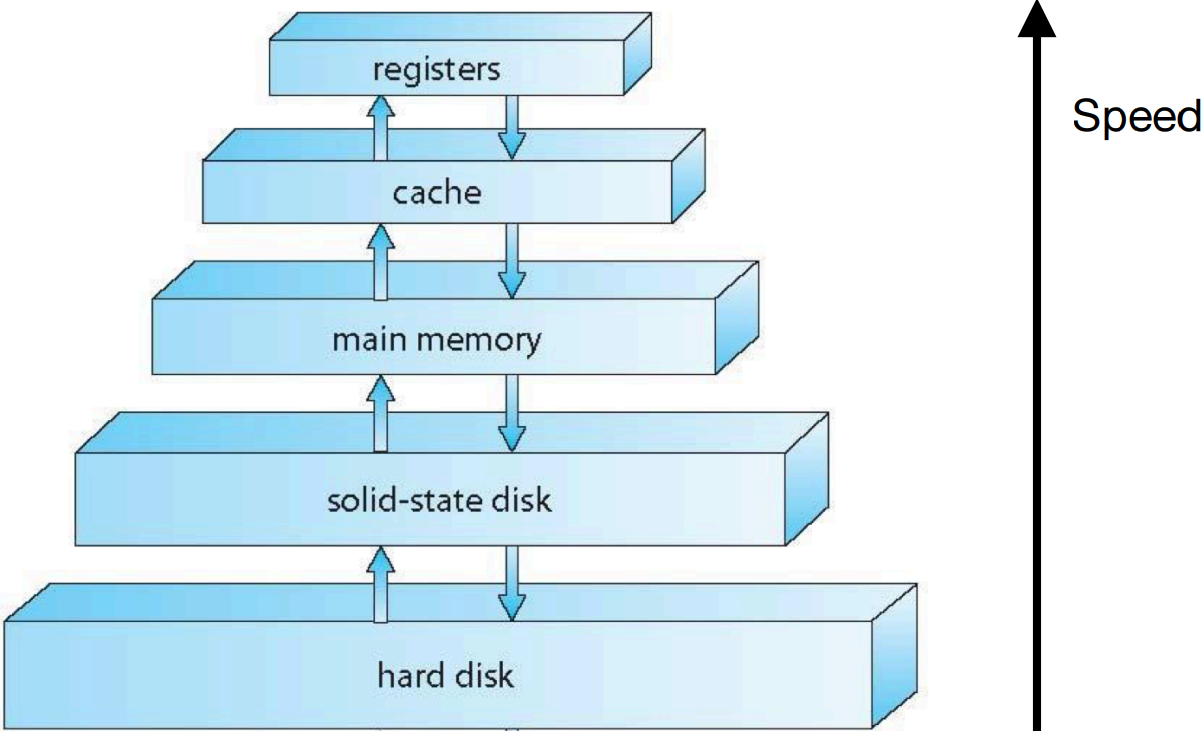
\includegraphics[scale=0.25]{img/mem.png}
\end{figure}

Without main memory and cache every time we have to access data we have to search it into
secondary memory, which is much slower.

\subsection{Performance of various levels of storage}


\begin{figure}[htbp]
    \centering
    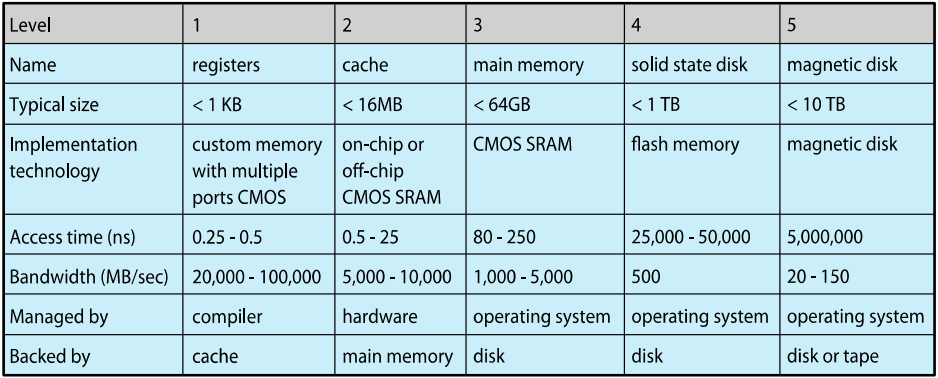
\includegraphics[scale=0.55]{img/stor.png}
\end{figure}

\newpage
\section{Modern system architectures: how a computer works}

First idea of a computer by Von Neumann is: Device comunicate with CPU and CPU comunicate with memory. This first idea is un-efficient because every input bother the CPU, so now device use the DMA (Direct Memory Access) to bypass CPU to send or to receve data directly to or from the main memory.

\begin{figure}[htbp]
    \centering
    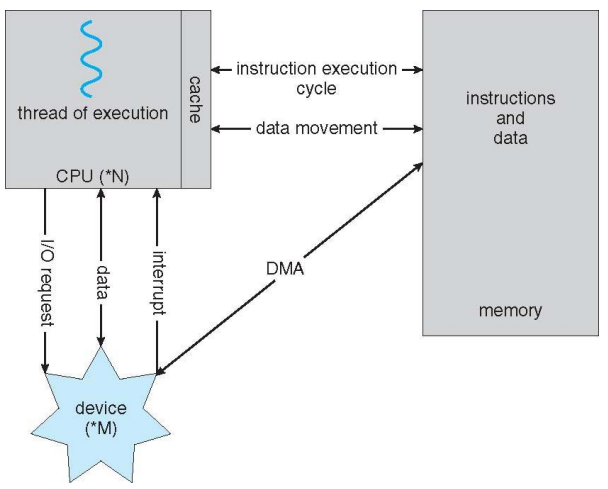
\includegraphics[width=0.65\linewidth]{img/cpu.png}    
\end{figure}


\subsection{Processor}

Lot of system use a single general-purpose processor. 
There are two different type of processors:

\begin{itemize}
    \item Multi-processor, each processor, with one core, has its own cache and register
    \item Multi-core, each core in the chip share cache and register with other core
\end{itemize}

\paragraph{}
Also there are two different way to work for multiple tasks:

\begin{itemize}
    \item Asymmetric processing (specific task)
    \item Symmetric processing (random tasks)
\end{itemize}


\subsubsection{Asymmetric Multi-processor}
Each processor, with one core each, is assigned a specific task. After performing the task, the processor waits another specific task and does not help other processors.

\subsubsection{Symmetric Multi-processor}
Each processor, with one core each, is assigned a random task. After performing the task, the processor helps the other processors and improves the overall performance.

\subsubsection{Asymmetric Multi-Core}
It is single chip, with several core inside. Each core works on a specific task and after performing the assigned specific tasks waits, without helping the other cores, for other specific tasks. 

\subsubsection{Symmetric Multi-Core}
It is single chip, with several core inside. Each core works on a random tasks and if one or more cores perform the task, the core helps the others, thus improving the overall performance.


\begin{figure}[htbp]
    \centering
    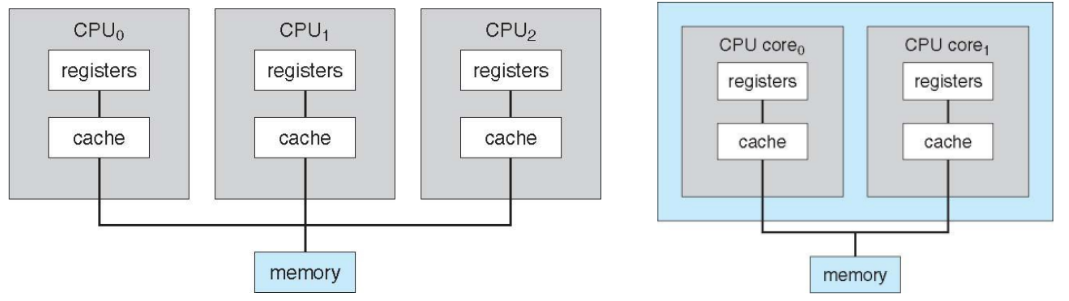
\includegraphics[width=1\linewidth]{img/multiP.png}
    \caption{Multi-processor on the left; Multi-Core on the right}
\end{figure}

\subsubsection{Is not it the same, why modern system are multi-core?}

\begin{itemize}
    \item On-Chip buses are faster;
    \item Single chip required less power;
    \item If one core die you throw the CPU in the bin
\end{itemize}

\subsection{High performance computer \textbf{HCP}}
If you do not care about power consumption and want a powerful machine because you are Google, Amazon etc., you should consider to build a Cluster.
A cluster is group of many computers, even with different OS, working together to complete tasks, such as cloud computing.
The application must be written to use parallelization.
\begin{figure}[htbp]
    \centering
    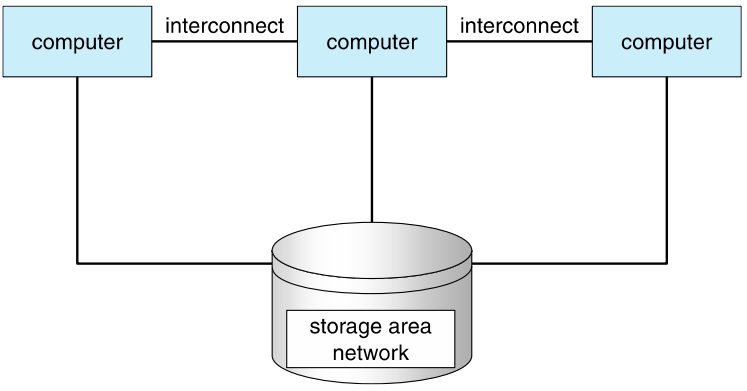
\includegraphics[width=0.6\linewidth]{img/SAN.png}
    \caption{SAN}
\end{figure}

Also Cluster server can chose with type of implementation to use:

\begin{itemize}
    \item Asymmetric: each machine has a hardware copy of the first machine, and if the first computer brakes the other machine, in hot-standby, starts working.
    \item Symmetric: has multiple nodes running applications, monitoring each other, if one brakes another machine takes its place.
\end{itemize}

\newpage

\section{Startup}
When you turn on the PC lots of things happen:

\begin{itemize}
    \item The bootstrap routine is invoked
    \item It stays in a pre-defined portion of the memory (firmware)
    \item The bootstrap routine initializes registers, memory and device controllers
    \item Calls the kernel and puts it in the main memory
    \item Starts daemons i.e., programs not in the kernel but that have to be run at startup like start and initialize driver for the monitor
    \item Once everything is ready, the OS is ready to provide an environment in which processes can be run
    \item A process is a program in execution
\end{itemize}

\subsection{Improve performance}


Executes multiple programs concurrently on a single CPU with one core need to improve efficiency.
There are two methods to improve performance: \textbf{Multiprogramming} and \textbf{Timesharing}


\subsubsection{Multiprogramming (Batch system)}

Think to have one processor with one core, system can not waste time, like wait for I/O. Multiprogramming organise tasks to do (code and data) so always CPU has something to do.
A subset of total jobs in system is kept in memory and when CPU has to wait (I/O), OS switches to another job.

Doesn't actually create the illusion of simultaneous execution for users.

\subsubsection{Timesharing (multitasking)}

Is logical extension in which CPU switches jobs so frequently that users can interact with each job while it is running, creating
interactive computing.
Users feel like they are interacting with their programs simultaneously, even though the CPU is only working on one program at a time.

We can also decide how to execute programs: by always finishing executing program-N or by starting to work first with the program that requires  the shortest execution time, or, like in the previous paragraph, by switching between different tasks.

\subsection{Switching Mechanism}

\subsubsection{Multiprogramming (Batch system)}

\begin{itemize}
    \item Relies on I/O events (like waiting for data from disk) to switch between processes.
    \item When the currently running program needs to wait for I/O, the CPU switches to another program that's ready to run.
\end{itemize}

\subsubsection{Timesharing (multitasking)}

\begin{itemize}
    \item Uses a time-slicing mechanism to switch between processes.
    \item The operating system allocates a short time slice (quantum) to each process, and after the quantum expires, it switches to the next ready process, regardless of its need for I/O.
\end{itemize}

In summary, while both multiprogramming and timesharing improve resource utilization, timesharing adds the concept of time slicing to create the illusion of simultaneous execution for multiple users, making it more user-friendly and interactive.


\newpage
\subsection{Security and OS protection}
Two different levels to interact with system function:

\begin{itemize}
    \item User mode (only some privileges decided by company or others admins)
    \item kernel mode (all privileges)
\end{itemize}

\begin{figure}[htbp]
    \centering
    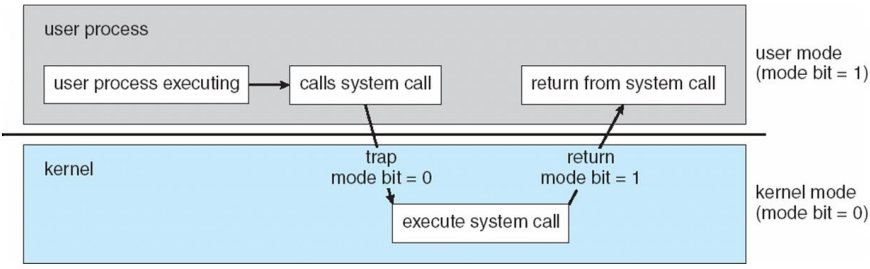
\includegraphics[width=0.8\linewidth]{img/secur.png}
\end{figure}

\paragraph{}
\begin{itemize}
    \item \textbf{Protection} – any mechanism for controlling access of processes or users to resources defined by the OS
    \item \textbf{Security} – defense of the system against internal and external attacks
\end{itemize}

System first distinguish users to determinate who can do what using: user IDs and group ID


An attach can threat to:
\begin{itemize}
    \item Confidentiality: absence of unauthorized disclosure of information
    \item Availability: service availability (CPU detect and stop malicious process)
    \item Integrity: absence of improper system alterations
\end{itemize}




\subsection{Program counter}
\begin{itemize}
    \item Single-threaded process has one program counter specifying location of next instruction to execute
    \item Multi-threaded process has one program counter per thread
\end{itemize}

\subsection{Storage Management}

OS provide to manage traffic data from RAM to SSD and vice versa, also OS give the impression that it is organise in directory.

\begin{itemize}
    \item \textbf{Multitasking} environments must be careful to use most recent
value, no matter where it is stored in the storage hierarchy
    \item \textbf{Multiprocessor} environment must provide cache coherency in
hardware such that all CPUs have the most recent value in their
cache
\end{itemize}


